\documentclass[12pt]{article}

\usepackage{fancyhdr} % Required for custom headers
\usepackage{float}
\usepackage{lastpage} % Required to determine the last page for the footer
\usepackage{extramarks} % Required for headers and footers
\usepackage{graphicx} % Required to insert images
\usepackage{amssymb}
\usepackage{enumerate}
\usepackage{svg}
\usepackage{hyperref}
\usepackage{caption}
\usepackage{subfig}


% Margins
\topmargin=-.5in
\evensidemargin=0in
\oddsidemargin=0in
\textwidth=6.5in
\textheight=9in
\headsep=0.25in
\graphicspath{{./figures/}}
\DeclareGraphicsExtensions{.jpg,.png,.svg}

\newcommand{\tab}{\hspace*{2em}}

\title{Combined Task and Motion Planner through an Interface Layer}
\author{Alex Gutierrez (ragtz@mit.edu), Bianca Homberg (bhomberg@mit.edu), \\and Veronica Lane (vmlane@mit.edu)}


%% ONE SENTENCE PER LINE TO MAKE THIS WORK NICELY IN GIT

\begin{document}

\maketitle 


\section{Testing}

\subsection{Baxter Robot}

We ran our test scenarios on the Baxter robot [Fig. \ref{fig:baxter}], designed by Rethink Robotics. 
Baxter is a humanoid robot with two 7 degree of freedom arms and a fixed based. 
Our tests used only the right arm with the two finger gripper.

\begin{figure}[h]
\centering
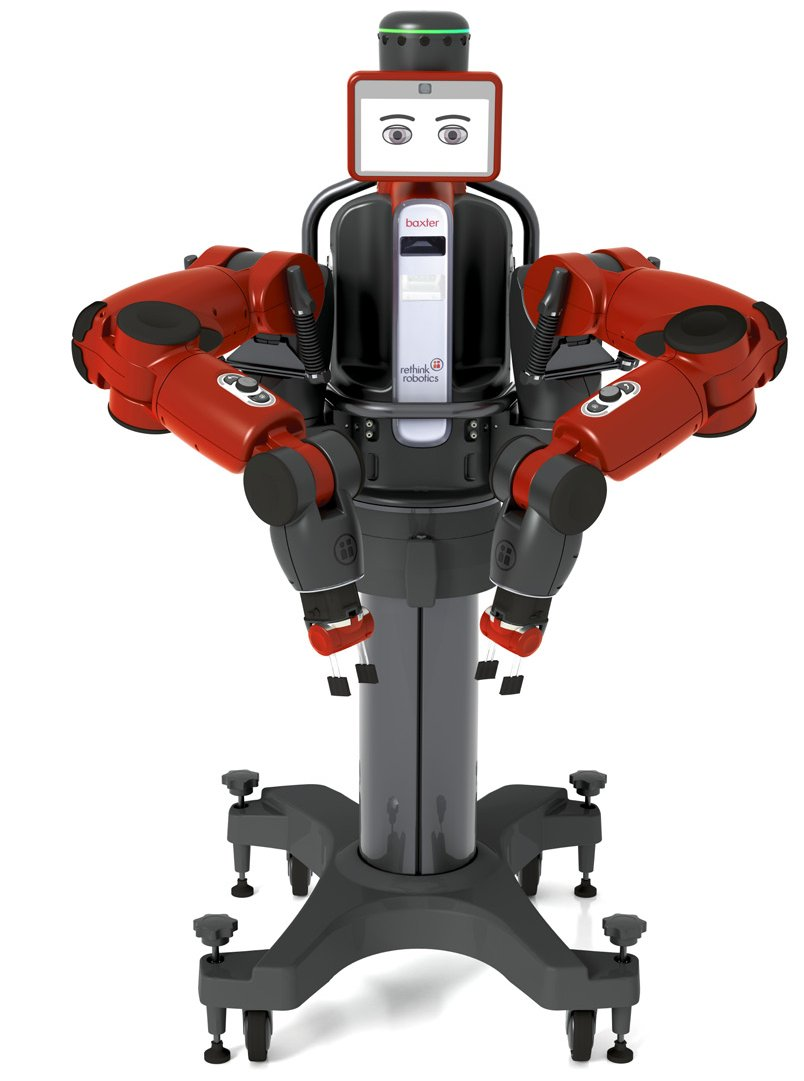
\includegraphics[width=.2\textwidth]{baxter}
\caption{The Baxter Robot \label{fig:baxter}}
\end{figure}

\subsection{Test Scenarios} \label{tests}

We present an interface between a task planner and a motion planner [2]. 
Baxter executes a variety of tests to measure the performance of the interface layer. 
The tests demonstrate that the interface layer respects all of the geometric constraints. 
Baxter picks up objects in a reasonable order to avoid collisions.

The goal of the first test is to move the object at the center of a $3\times3$ square grid of objects to a goal surface. 
In order to achieve the goal, Baxter must move some of the blocks surrounding the center block before placing the center block on the target surface.
The goal of the second test is to sort red, green, and blue blocks into separate bins.
For this task, the high level plan must ensure that Baxter does not try to pick up a block that is surrounded by other blocks.
Figure \ref{fig:scenarios} shows the setup of the different test scenarios. 

\begin{figure}[h]
\centering
\def\svgwidth{.4\textwidth}
\input{figures/scenarios.pdf_tex}
\caption{Set up of test scenarios.\label{fig:scenarios}}
\end{figure}

\section{Technical Approach}
Through the use of the interface layer implemented in the previous problem set, a task planner can operate in a geometry-independent abstract state space while handling geometric constraint discovery and requisite replanning via communication between the interface layer and the task and motion planners. 

The interface layer was implemented in python as a ROS package, which is set up to communicate with user-implemented task and motion planners via the client/server paradigm. 
More specifically, the task and motion planners were implemented as ROS services. 
The interface layer acts as client to both of these services. 
Figure \ref{fig:blockDiagram} diagrams the system framework.

Given that the pose generation and state update vary between domains, we implement domain specific pose generator class and state update function for the scenarios described in Section \ref{tests}.

%The three components of our combined task and motion planner system are:  \(1\) the task planner, \(2\) the motion planner, and \(3\) the interface layer. 
%The interface layer is composed of the state update and pose generator modules [Fig. \ref{fig:blockDiagram}].

\begin{figure}[h]
\centering
\def\svgwidth{0.7\textwidth}
\input{figures/blockDiagram.pdf_tex}
\caption{System Block Diagram\label{fig:blockDiagram}}
\end{figure}

\subsection{Task Planner}
We used the FF task planner [1]. 
Our software for the task planner is the same as the previous problem set. 
The task planner is instantiated with a given PDDL domain file.  
As a ROS service, it takes in a PDDL problem specification of current state and goal from the interface layer. 
It returns a set of actions leading to the desired goal state. 

\subsection{Motion Planner}
We used the MoveIt! motion planner [3]. 
We implenented a ROS service wrapper for this off-the-shelf motion planner so as to comply with the API.
It takes as input the state of the world, the action to be performed, and a pose goal (i.e. a series of waypoints to perform the action).
MoveIt! is then used to instantiate motion plans between these waypoints. 
The motion planner service returns a boolean specifying the success or failure of the instantiation of the motion plan, the motion plan itself, and the updated world state (which can be unchanged if the action failed).

\subsection{Interface}

\begin{figure}[t]
\centering
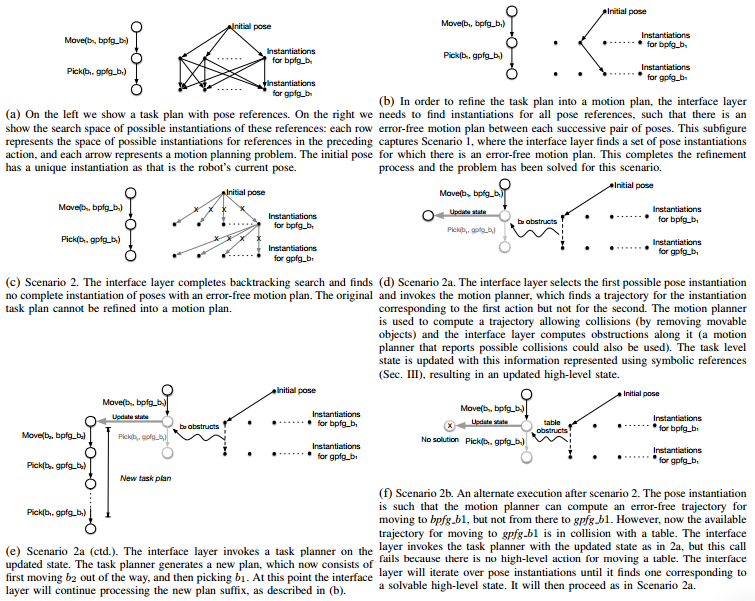
\includegraphics[width=\textwidth]{figure4}
\caption{Illustration of the interface layer’s refinement process. 
Action arguments have been abbreviated. 
Taken from [2]
\label{fig:figure4}}
\end{figure}

\subsubsection{Algorithm 1}

\begin{figure}[t]
	\centering
	\subfloat{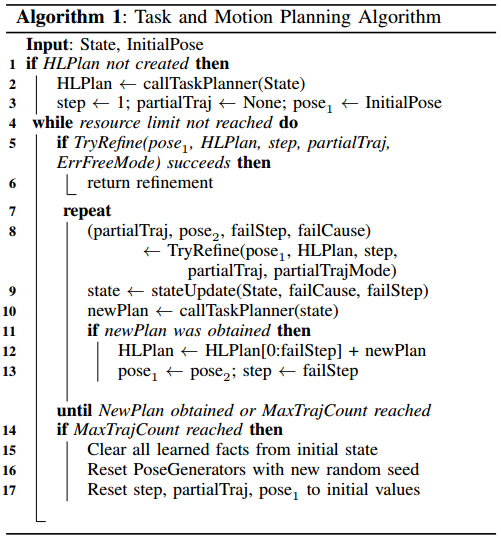
\includegraphics[width=.45\linewidth]{algorithm1}}
	\qquad
	\subfloat{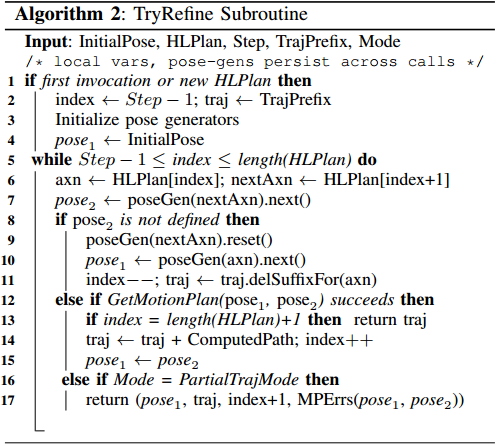
\includegraphics[width=.45\linewidth]{algorithm2}}
	\caption{Pseudo-code for the underlying algorithms of the interface layer. Taken from [2]\label{fig:algorithms}}
\end{figure}

We start with an initial state where no objects obstruct any motions.  
From there, we look for a high level plan.  
If we succeed at finding a high level task plan, we begin the process of attempting to find a motion corresponding to each action.

First, we start by attempting to find a full refinement of the whole plan, calling the TryRefine subroutine in error-free mode.  
If that succeeds, then we return the plan.  

If that does not succeed, we find a partial trajectory that goes as far as it can by calling the TryRefine subroutine in partial trajectory mode.  
This function returns a partial trajectory along with the step where it failed and the determined cause for failure.  
Then, we update the state based on the actions up until that point and add in the obstructing obstacles corresponding to the failure.  
Now, we attempt to find a new high level plan, and iterate.  

If we fail to find a new high level plan at any point, we re-run the TryRefine subroutine on the original high level plan from the previous step.  
Since the TryRefine subroutine has randomization from pose generators, re-running it may yield a better solution. 

We have several checks where, if we fail to find a solution, we clear all of our information and start over.  
Due to the randomization of the pose generators, we may make better choices during subsequent iterations.  

Every time a new partial plan is generated, we first try to fill it completely using backtracking search (calling TryRefine in error-free mode) before giving up and resorting to the partial trajectory finding.  

\subsubsection{Algorithm 2}


In the TryRefine subroutine, the interface layer attempts to find motion plans corresponding to the various actions.  
It has two modes: error free and partial trajectory.  
In error free mode, it performs backtracking search to try to find a full plan from start to finish.  

In partial trajectory mode, TryRefine goes as far as it can, but when it finds an infeasible motion plan for some action, it returns the step at which it failed.  
In addition to returning the failed step, it returns the cause of the errors.  
The function MPErrs removes various objects from the environment until it find a plan which succeeds.  
It then marks all of those objects which were removed as blocking objects.

As described above in Algorithm 1, once the list of blocking objects is returned, the interface layer updates the state and attempts to replan from there.

\subsubsection{State Update}

When an action is infeasible because an object is blocking another object, the interface layer updates the state and calls the task planner. 
The interface layer, as described above, determines a list of obstructing objects.
The state update function goes through a section of a high level plan, performing all of the actions and updating the current state of the world.
Once the state update function reaches the step where the TryRefine function failed, the state update function adds predicates to the state describing which blocks obstruct other blocks.
The state function updates each action based on the preconditions and postconditions of each action: it confirms that all of the preconditions are satisfied and then adds true postconditions and removes falsified postconditions.  

For instance, for the PICKUP action, the state update functions confirms that the gripper is empty, adds the postcondition that the gripper is full and that the object is in the gripper and removes the postcondition that the object is on whichever surface it started on.
%If the object is movable, the task planner will generate a plan to move the object out of the way before moving the target object. 
%If the object is not movable, such as the table, the interface will perform backtracking search to try to find a full plan from start to finish.
%The backtracking search is over possible pose instantiations: since some poses may be infeasible and since previous choices may affect future choices, the backtracking search iterates over all possible poses in order to find a full solution if a full solution exists. 

%Every time a new partial plan is generated, we first try to fill it completely using backtracking search before giving up and resorting to the partial trajectory finding.  
%In our manipulation example, the interface tries to pick up blocks from all angles before giving up and assuming they must be blocked by something.  

\subsubsection{Pose Generator}

When the pose generator is called by the interface layer, it generates a set of random poses for each action. 
Each pose is made up of a set of waypoints. 
We generate multiple waypoints for an action to ensure that the motions avoid collisions.

For the PICKUP action, it generates the following waypoints: a pre-grasp near the object and pointing towards it, touching the object, grasping the object, lifting the object, and a standard home position. 
The pre-grasp is randomly generated and places the gripper about 15 centimeters away from the object.
We divided the set of possible random yaw angles around the object into several distinct ranges, called \textit{slices}. 
Each call to the pose generator generates a random angle in one of the ranges.
The second waypoint moves the arm so that the object is in the gripper. 
The grasping waypoint is in the exact same position with the gripper closed. 
The lifting waypoint is directly above the grasping waypoint, high enough so that the object is above all of the other objects on the table. 
Finally, the last waypoint goes to the standard home position. 

For the PUTDOWN action, the pose generator generates the following waypoints: above the target location, a set down position with the gripper closed, a set down position with the gripper open, 15 cm backed away from the target location, and the standard home position. 
The target location is randomly generated, but the pose generator checks to make sure that no objects are at or near the target location.

For the sorting task, the PUTDOWN pose generator behaves slightly differently, since objects are dropped into bins rather than placed.
In this case, the pose generator had a fixed specified location to drop the object and had no randomization.

To reiterate, a pose is a set of waypoints. 
The pose generator keeps track of the number of poses it has generated, at least one for each slice. 
Once the pose generator has generated the maximum number of poses, it returns None, to indicate that no poses are feasible. 
The interface layer then backtracks and resets the pose generator. 
The TryRefine method of the interface layer attempts to generate a feasible motion plan between each pose.  
The motion planner is called to create this motion plan, including motion plans between waypoints.

\section{Improvements}

We implemented a number of improvements in order to increase the efficiency of the algorithm.

\subsection{Error-free mode}

The original version of the algorithm, as shown in \ref{fig:algorithms}, only attempts to find partial trajectories when it replans partway through the procedure.  
For our version of the algorithm, every time a new partial plan is generated, we first try to instantiate it completely using backtracking search (calling TryRefine in error-free mode) before giving up and resorting to the partial trajectory finding. 

This enables us to find plans a lot more quickly: whenever a plan is possible, we find it by backtracking search.  
Often, the first pose that is tried will not be viable but another pose will.  
Partial trajectory mode will only try the first pose before giving up and identifying blocking objects.
If partial trajectory mode is continually used, then often the plans created are much longer than necessary just because an invalid first pose is chosen when other options would have worked fine.
Using the full backtracking search on each new high level plan avoids this problem.

\subsection{Motion Planner Collision Heuristic}

We added a heuristic to avoid motion planner calls in cases where we could easily determine that it would fail.
Specifically, the motion planner service would use the world geometry and basic collision geometry to determine if the pose obviously would cause the robot arm to intersect with obstacles.
This greatly increased the efficiency for planning in crowded environments since it enabled the motion planner to return a fail much more quickly, rather than trying the full planning procedure when the end goal wasn't reachable. 

\subsection{O(n) Identification of Obstructions}

To find the blocking objects, we start by iterating through a randomized list of the objects.  
We continue removing objects until we find a successful motion plan.  
We will eventually find a successful motion plan since if there are no other objects in the world, the motion should succeed.  
After we find this possible list of removed objects, we iterate through all of the objects we removed.  
We attempt to add these objects in one by one, leaving added in all of those which do not obstruct our found motion plan.  
This leaves us with a local minimum of removed objects: it may be possible to find another smaller set of objects that, if removed, allow a valid motion plan.  
However, for this set of objects, no object can be added back in without obstructing the motion plan.
This algorithm for determining obstructing objects is $O(n)$.

The paper originally describes an $O(n^2)$ algorithm for determining obstructing objects, starting by removing each individual object, then pairs of objects, etc.  
This ensures a minimum removal set but requires significantly more motion planner calls.

\subsection{Future Improvements}

The interface layer winds up making a lot of duplicate calls to the motion planner.
If the interface layer kept track of more state, perhaps via some memoization process of poses and actions, it would be able to save a lot of motion call attempts.
Furthermore, when the interface layer finds obstructing objects, it finds obstructing objects for a particular pose.  
If that pose were stored, then the interface layer would never attempt to use a different pose which might have different blocking objects, and would instead directly use the pose that the plan was optimized for.


\section{Results}
\subsection{Metrics}
We measured the performance of each test by the runtime and the number of calls to both the task planner and motion planner [Fig. \ref{benchmark}]. 
The interface layer is designed to be independent of any specific task and motion planner libraries, therefore the number of calls to the motion and task planner measures the performance of the interface layer better than the total runtime. 
The actual runtime depends on the motion planner and task planner chosen.

\subsection{Square Grid}
We ran the square grid scenario on a simulated Baxter robot.
The planner took approximately an hour to find a feasible plan. 
In simulation, Baxter successfully moves blocks to reach the target center block and places the center block on the target surface.
A video of the successful test trial in simulation can be found at \url{http://youtu.be/Jb9EOZ8B2lU}.  
We did not run this test on the real Baxter robot.

\subsection{Sorting}
We ran the sorting task in simulation and on the physical Baxter robot.
The planner took approximately twenty minutes to find a feasible plan. 
We ran many test trials to achieve a successful run because the system was open-loop with respect to the environment.
It had feedback on the world position of the arms, but not on the position of the arms relative to the objects. This mean that drift accumulated over time.
Additionally, the Baxter arm is shaky, and without very much room for error in the motion plans, Baxter sometimes hit adjacent objects due to wobbling outside of the planned motion.
Baxter successfully sorts green, red, and blue blocks into different bins. 
A video of the successful test trial can be found at \url{http://youtu.be/445_t_lUBdU}.

\begin{figure}
\begin{tabular}[t]{|l|l|l|l|l|l|l|}
\hline

Task & Trial & \shortstack{Number of \\Blocks} &\shortstack{Blocks to Move} & \shortstack{Number of \\TP Calls} & \shortstack{Number of \\MP Calls} & Runtime (min) \\ \hline
Square Grid & 1 & 9 & 1 & 3 & 721 & 21.45\\
\hline
 & 2 &  &  & 3 & 1376 & 86.98\\
\hline
 & 3 &  &  & 3 & 1198 & 80.11\\
\hline
 & \textbf{Avg} &  &  & \textbf{3} & \textbf{1098.33} & \textbf{62.85}\\
 
\hline
Sorting & 1 & 9 & 9 & 8 & 353 & 22.33\\
\hline
 & 2 &  &  & 6 & 304 & 15.97\\
\hline
 & 3 &  &  & 6 & 379 & 20.76\\
 \hline
 & \textbf{Avg} &  &  & \textbf{6.67} & \textbf{345.33} & \textbf{19.69}\\

\end {tabular}
\caption{Test Scenarios Performance}
\label{benchmark}
\end{figure}

\section{Limitations}

The interface does not scale well to large object state spaces, as this increases the number of geometric constraints. 
This increase in geometric constraints causes the number of motion planner calls to explode, slowing down the planning stage. 
In addition, in its current implementation it only works within deterministic, fully-observable environments and is not suitable for online replanning.

\section{Code}

The code for pset 4 is available at \url{https://github.com/bhomberg/6834-task-motion-planner}.

\section{References}

\hspace{.25in}[1] J. Hoffmann, B. Nebel. ``The FF planning system: fast plan generation through heuristic search''. J. Artif. Int. Res. 14, 1, 253-302, 2001.

[2] S. Srivastava, E. Fang, L. Riano, R. Chitnis, S. Russell, P. Abbeel. ``Combined Task and Motion Planning Through an Extensible Planner-Independent Interface Layer''. IEEE International Conference on Robotics and Automation (ICRA), 2014.

[3] I. A. Sucan and Sachin Chitta, ``MoveIt!''. [Online] Available: \url{http://moveit.ros.org}

\end{document}

